\documentclass[12pt]{article}

\usepackage{amsmath,amsthm,amsfonts,amssymb,amsxtra}
\usepackage{pgf,tikz}
\usetikzlibrary{arrows}
\renewcommand{\theenumi}{(\alph{enumi})} 
\renewcommand{\labelenumi}{\theenumi}

\pagestyle{empty}
\setlength{\textwidth}{7in}
\setlength{\oddsidemargin}{-0.5in}
\setlength{\topmargin}{-1.0in}
\setlength{\textheight}{9.5in}

\theoremstyle{definition}
\newtheorem{problem}{Problem}

\begin{document}

\noindent{\large\bf MATH 142}\hfill{\large\bf Exam \#2.}\hfill{\large\bf
  Fall 2016}\hfill{\large\bf Page 1/6}\hrule

\bigskip
\begin{center}
  \begin{tabular}{|ll|}
    \hline & \cr
    {\bf Name: } & \makebox[12cm]{\hrulefill}\cr & \cr
    {\bf VIP ID:} & \makebox[12cm]{\hrulefill}\cr & \cr
    \hline
  \end{tabular}
\end{center}
\begin{itemize}
\item Write your name and your VIP ID in the space provided above.
\item The test has six (6) pages, including this one.
\item Enter your answer in the box(es) provided.
\item You must show sufficient work to justify all answers unless
  otherwise stated in the problem.  Correct answers with inconsistent
  work may not be given credit.
\item Credit for each problem is given in parentheses at the right of
  the problem number.
\item No books, notes or calculators may be used on this test.
\end{itemize}
\hrule

\begin{tabular}{ll}

\begin{tikzpicture}
\draw (0,0) node [scale=0.6]{
  \begin{tabular}{|c|c|c|}
    \hline
    &&\cr
    {\large\bf Page} & {\large\bf Max.~points} & {\large\bf Your points} \cr
    &&\cr
    \hline
    &&\cr
    {\Large 2} & \Large 20 & \cr
    &&\cr
    \hline
    &&\cr
    {\Large 3} & \Large 20 & \cr
    &&\cr
    \hline
    &&\cr
    {\Large 4} & \Large 30 & \cr
    &&\cr
    \hline
    &&\cr
    {\Large 5} & \Large 20 & \cr
    &&\cr
	\hline
    &&\cr
    {\Large 6} & \Large 10 & \cr
    &&\cr
    \hline\hline
    &&\cr
    {\large\bf Total} & \Large 100 & \cr
    &&\cr
    \hline
  \end{tabular}};
\end{tikzpicture}  &
\raisebox{-0.4\height}{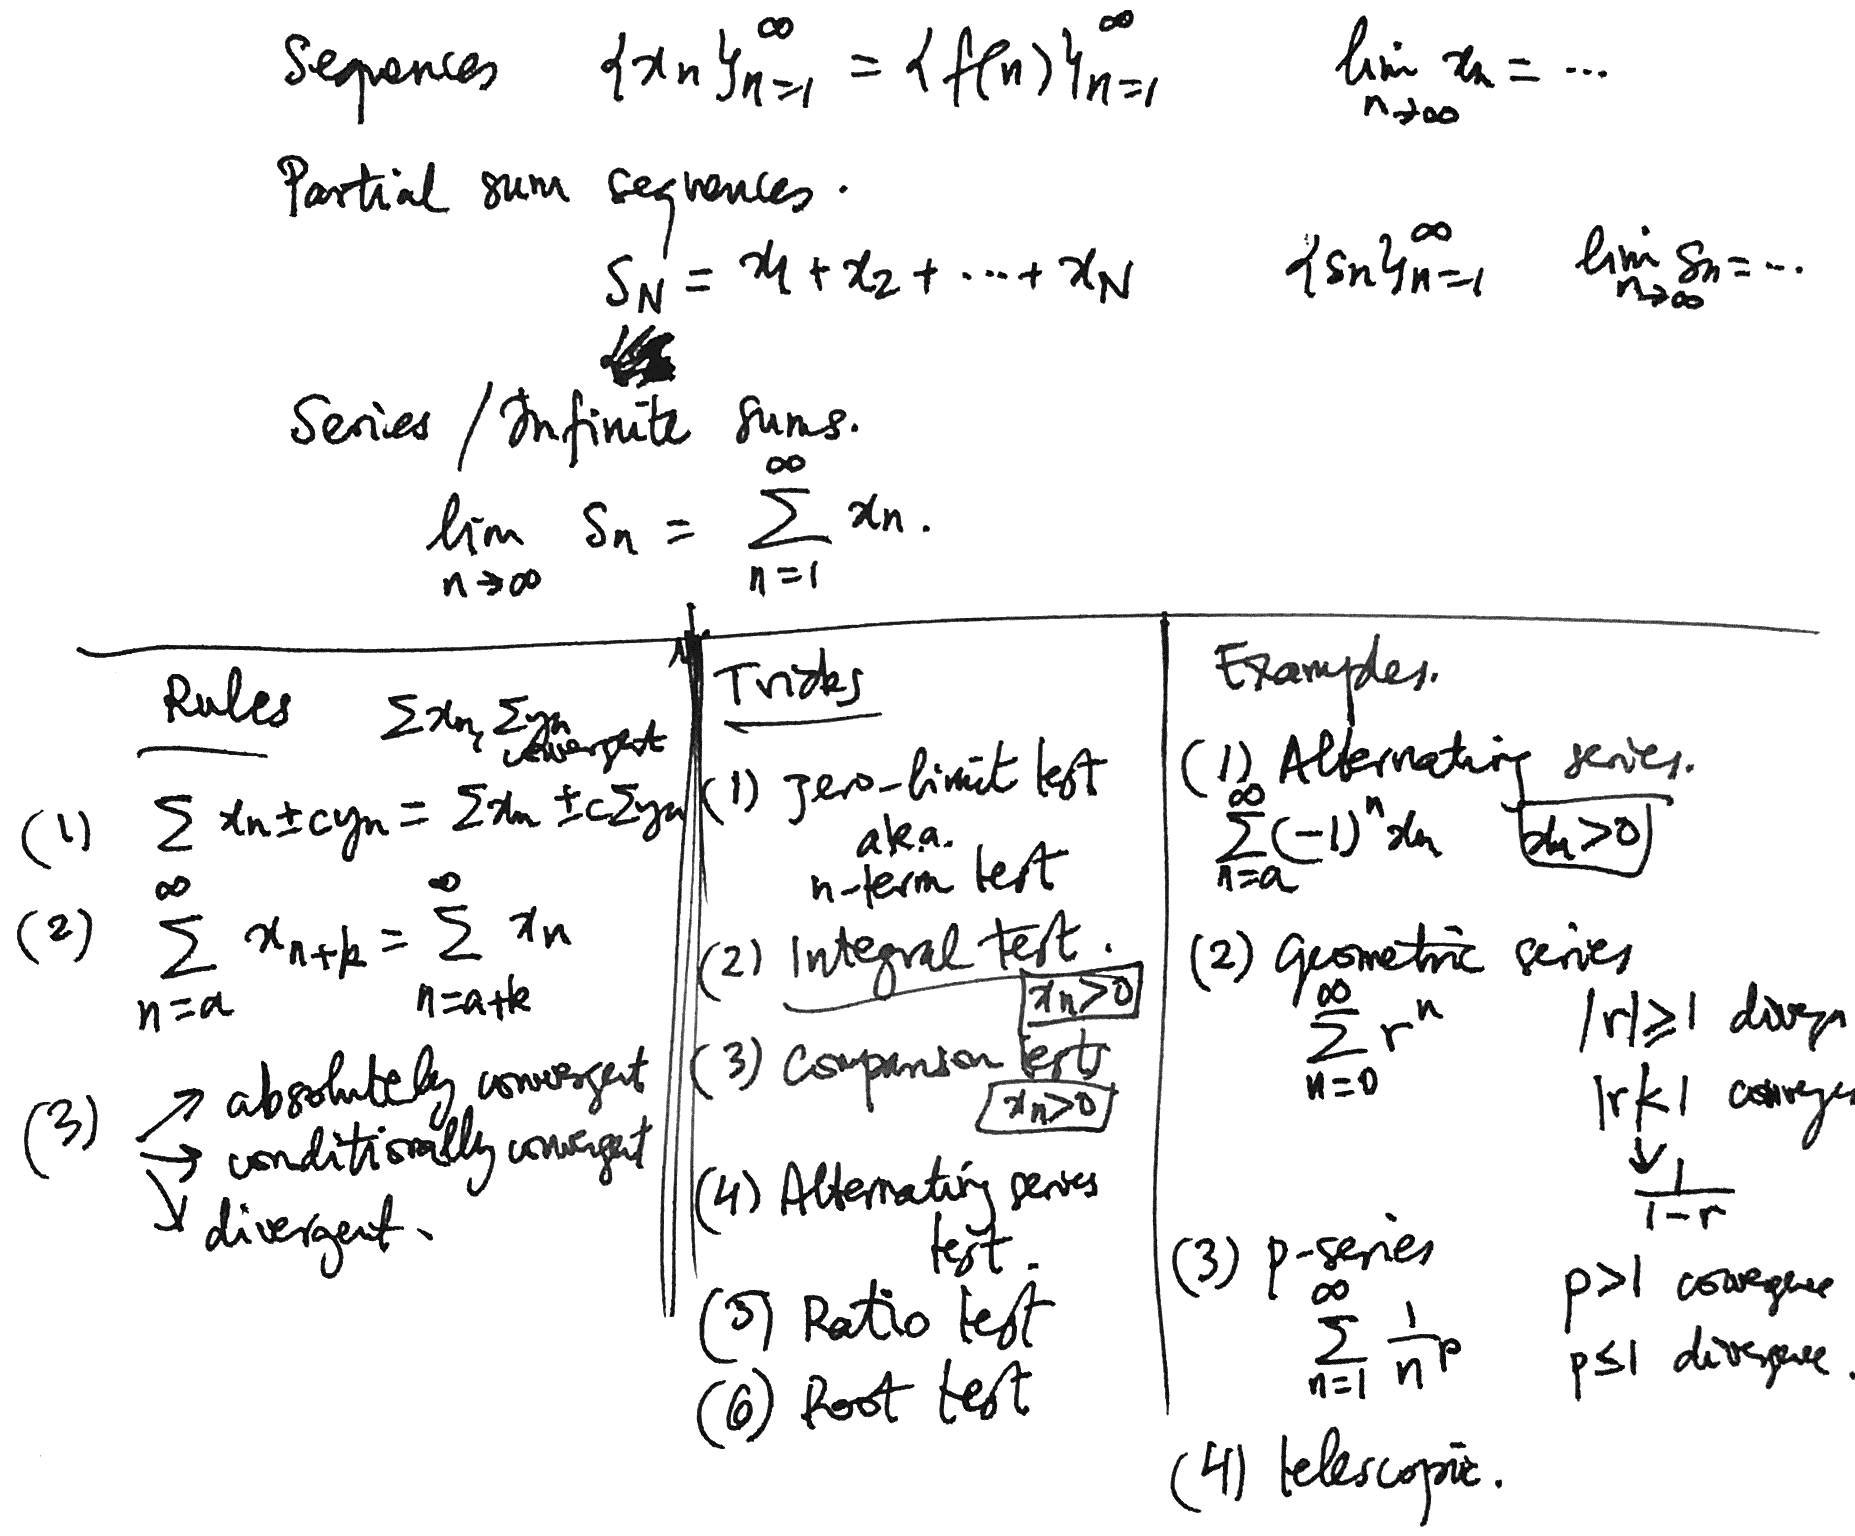
\includegraphics[width=0.75\linewidth]{wdwn.png}}
\end{tabular}
\newpage

%%%%%%%%%%%%%%%%%%%%%%%%%%%%%%%%%%%%% Page 2
\noindent{\large\bf MATH 142}\hfill{\large\bf Exam \#2.}\hfill{\large\bf
  Fall 2016}\hfill{\large\bf Page 2/6}\hrule

\bigskip
{\problem[10 pts---5 pts each part] Find a formula for the general term of the following sequences:} 
\begin{enumerate}
\item $\displaystyle{\frac{1}{2}, \frac{3}{4}, \frac{5}{6}, \frac{7}{8}, \dotsc}$
\bigskip
\begin{flushright}
  \begin{tikzpicture}
    \draw (-0.5cm,0.5cm) node {$x_n = $};
    \draw (0cm,-0.2cm) rectangle (5cm,1.2cm);
  \end{tikzpicture}
\end{flushright}
\item $\displaystyle{1-\frac{1}{2}, \frac{1}{3} - \frac{1}{2}, \frac{1}{3} - \frac{1}{4}, \frac{1}{5}-\frac{1}{4}, \dotsc}$
\vspace{3cm}
\begin{flushright}
  \begin{tikzpicture}
    \draw (-0.5cm,0.5cm) node {$x_n = $};
    \draw (0cm,-0.2cm) rectangle (5cm,1.2cm);
  \end{tikzpicture}
\end{flushright}
\end{enumerate}
\hrule
{\problem[10 pts---5 pts each part] Write out the first five terms of the sequence $\left\{ \displaystyle{\frac{(-1)^{n+1}}{n^2}} \right\}_{n=1}^\infty$ \newline Determine whether the sequence converges, and if so find its limit.
\vspace{7cm}
\begin{flushright}
  \begin{tikzpicture}
    \draw (-5.75cm,1.9cm) node {First five terms:};
    \draw (-4cm, 1.3cm) rectangle (5cm, 2.7cm);
    \draw (-1.25cm,0.5cm) node {$\displaystyle{\lim_{n \to \infty} x_n} = $};
    \draw (0cm,-0.2cm) rectangle (5cm,1.2cm);
  \end{tikzpicture}
\end{flushright}
\newpage


%%%%%%%%%%%%%%%%%%%%%%%%%%%%%%%%%%%%% Page 3
\noindent{\large\bf MATH 142}\hfill{\large\bf Exam \#2.}\hfill{\large\bf
  Fall 2016}\hfill{\large\bf Page 3/6}\hrule

\bigskip
{\problem[20 pts---10 pts each]  Determine whether the series converge, and if so find their sum:}
\begin{enumerate}
\item $\displaystyle{\sum_{n=1}^\infty 5\Big( \frac{3}{4} \Big)^{n-1}}$ 

(\textbf{Hint:} This looks like a geometric series)
\vspace{7cm}
\begin{flushright}
  \begin{tikzpicture}
    \draw (-1.75cm,0.5cm) node {$\displaystyle{\sum_{n=1}^\infty 5 \Big( \frac{3}{4} \Big)^{n-1} }= $};
    \draw (0cm,-0.2cm) rectangle (5cm,1.2cm);
  \end{tikzpicture}
\end{flushright}
\item $\displaystyle{\sum_{n=1}^\infty \frac{1}{(n+2)(n+3)}}$

(\textbf{Hint:} This is a telescopic series. Partial fraction decomposition is your friend here)
\vspace{7cm}
\begin{flushright}
  \begin{tikzpicture}
    \draw (-2cm,0.5cm) node {$\displaystyle{\sum_{n=1}^\infty \frac{1}{(n+2)(n+3)}  }= $};
    \draw (0cm,-0.2cm) rectangle (5cm,1.2cm);
  \end{tikzpicture}
\end{flushright}
\end{enumerate}
\newpage

%%%%%%%%%%%%%%%%%%%%%%%%%%%%%%%%%%%%% Page 4
\noindent{\large\bf MATH 142}\hfill{\large\bf Exam \#2.}\hfill{\large\bf
  Fall 2016}\hfill{\large\bf Page 4/6}\hrule

\bigskip
{\problem[10 pts]  Apply the \textbf{zero-limit test} (also known as
  the divergence, or the $n$-term test) and state what it tells you about the series.}
\begin{equation*}
\sum_{n=1}^\infty \frac{n^2+n+3}{2n^2+1}.
\end{equation*}
\vspace{2cm}
\hrule
{\problem[10 pts]  Use the \textbf{integral test} to determine
  whether the series $\displaystyle{\sum_{n=1}^\infty \frac{1}{5n+2}}$
  converges.} 
\vspace{6.5cm}
\hrule
{\problem[10 pts]  Use the \textbf{ratio test} to determine whether
  the series $\displaystyle{\sum_{n=1}^\infty (-1)^n \frac{4^n}{n^2}}$  
  converges.  If the test is inconclusive, then say so.} 
\newpage

%%%%%%%%%%%%%%%%%%%%%%%%%%%%%%%%%%%%% Page 5
\noindent{\large\bf MATH 142}\hfill{\large\bf Exam \#2.}\hfill{\large\bf
  Fall 2016}\hfill{\large\bf Page 5/6}\hrule
  
\bigskip

{\problem[10 pts]  Use the \textbf{root test} to determine whether
  the series $\displaystyle{\sum_{n=1}^\infty \Big( \frac{3n+2}{2n-1}
    \Big)^n}$ converges.  If the test is inconclusive, then say so.} 
\vspace{9cm}
\hrule{\problem[10 pts]  Classify the series
  $\displaystyle{\sum_{n=1}^\infty (-1)^n\, \frac{4n^2+1}{n!}}$ as
  absolutely convergent, conditionally convergent, or divergent.} 

\newpage

%%%%%%%%%%%%%%%%%%%%%%%%%%%%%%%%%%%%% Page 6
\noindent{\large\bf MATH 142}\hfill{\large\bf Exam \#2.}\hfill{\large\bf
  Fall 2016}\hfill{\large\bf Page 6/6}\hrule
{\problem[10 pts]  Use any of the \textbf{comparison tests} to determine the
  convergence of the series}
\begin{equation*}
\sum_{n=0}^\infty \frac{3^n}{5^{n+1}+4}
\end{equation*}

\end{document}
